\chapter{Basic Operations in Riemannian Space}
\pagebreak[4]

\section{p27-exercise}

\begin{tcolorbox}
Take polar coordinates $r, \theta$ in a plane. Draw the infinitesimal triangle with vertices $(r,\theta)$, $(r+dr,\theta)$, $(r,\theta + d\theta)$. Evaluate the square on the hypotenuse of this infinitisimal triangle, and so obtain the metric tensor for the plan for the coordinates$(r, \theta)$.\end{tcolorbox}
\begin{figure}[htp] 
    \centering
\includegraphics[scale=.5]{polar.jpg}
\end{figure}
 
\begin{align} 
\ ds^2 &= |AB|^2\\
\ &= dr^2 +|CA|^2\\
\ |CA| &= r\sin(d\theta)\approx rd\theta\\
\Rightarrow ds^2 &= dr^2 + r^2d\theta^2\\
\Rightarrow (a_{mn}) &= \begin{pmatrix}
 1& 0 \\
0 & r^2 \\
\end{pmatrix}
\end{align}

$$\medblackdiamond$$
\pagebreak[4]

\section{p27-exercise}

\begin{tcolorbox}
Show that if $x^1 = r, x^2 = \theta, x^3 = \phi$, in the usual notation of spherical polar coordinates, then $$ a_{11} =1, a_{22} = r^2, a_{33} = r^2\sin^2\theta$$ and the other components vanish.
\end{tcolorbox}
\begin{figure}[h]
\centering
\begin{minipage}[t]{.5\textwidth}
%\centering
\vspace{0pt}
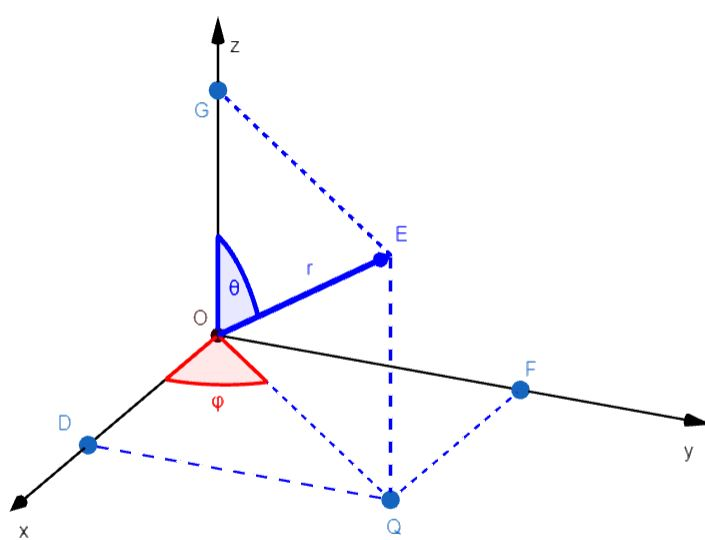
\includegraphics[scale=.5]{spherical.jpg}
\end{minipage}\hfill
\begin{minipage}[t]{0.4\textwidth}
%\centering
\vspace{50pt}
We use the latitude $\psi$ instead of the co-latitude $\phi$.\\\\
$\left\{ \begin{array}{c}
    x= r\cos (\psi )\cos (\theta) \\
     y= r\cos (\psi )\sin (\theta) \\
      z= r\sin(\psi )
  \end{array} \right.$
\end{minipage}
\end{figure}
\begin{align} 
\ ds^2 = dx^2 + dy^2 + dz^2\quad\text{with}\\
\left.
\begin{array}{c}
    dx= dr\cos (\psi )\cos (\theta)- r\sin (\psi )d\psi\cos (\theta) -r\cos (\psi )\sin (\theta)d\theta\\
     dy= dr\cos (\psi )\sin (\theta) -r\sin (\psi )d\psi\sin (\theta)+r\cos (\psi )\cos (\theta)d\theta\\
      dz= dr\sin(\psi )+r\cos(\psi )d\psi\\
  \end{array} \right\}
  \end{align}
  \begin{align}
  \left.
  \begin{array}{c}
    dx^2=
    \cos^2 (\psi )\cos^2 (\theta)dr^2\\- r^2\sin^2 (\psi )\cos^2 (\theta)d\psi^2\\ -r^2\cos^2 (\psi )\sin^2 (\theta)d\theta^2\\
    -\cos (\psi )\cos (\theta) r\sin (\psi )\cos (\theta)drd\psi\\
    -\cos (\psi )\cos (\theta)r\cos (\psi )\sin (\theta)drd\theta\\
    +r\sin (\psi )\cos (\theta)r\cos (\psi )\sin (\theta)d\psi d\theta  \\\\
     dy^2=  \cos^2 (\psi )\sin^2 (\theta)dr^2\\ +r^2\sin^2 (\psi )\sin^2 (\theta)d\psi^2\\+r^2\cos^2 (\psi )\cos^2 (\theta)d\theta^2\\-\cos (\psi )\sin (\theta)r\sin (\psi )\sin (\theta)dr d\psi\\ - \cos (\psi )\sin (\theta)r\cos (\psi )\cos (\theta)drd\theta\\
     -r\sin (\psi )\sin (\theta)r\cos (\psi )\cos (\theta)d\psi d\theta\\\\
      dz^2= \sin^2(\psi )dr^2 +r^2\cos^2(\psi )d\psi^2 + r\sin(\psi )\cos(\psi )drd\psi\\
  \end{array} \right\}
\end{align}
Rearrange terms:
  \begin{align}
  \left.
  \begin{array}{c}
    dx^2=
    \cos^2 (\psi )\cos^2 (\theta)dr^2\\+ r^2\sin^2 (\psi )\cos^2 (\theta)d\psi^2\\ +r^2\cos^2 (\psi )\sin^2 (\theta)d\theta^2\\
    -r\cos (\psi )\sin (\psi )\cos^2 (\theta)drd\psi\\
    -r\cos^2 (\psi )\cos (\theta)\sin (\theta)drd\theta\\
    +r^2\sin (\psi )\cos (\theta) \cos (\psi )\sin (\theta)d\psi d\theta  \\\\
     dy^2=  \cos^2 (\psi )\sin^2 (\theta)dr^2\\ +r^2\sin^2 (\psi )\sin^2 (\theta)d\psi^2\\+r^2\cos^2 (\psi )\cos^2 (\theta)d\theta^2\\-r\cos (\psi )\sin (\psi )\sin^2 (\theta)dr d\psi\\ - r\cos^2 (\psi )\sin (\theta) \cos (\theta)drd\theta\\
     -r^2\sin (\psi )\sin (\theta)\cos (\psi )\cos (\theta)d\psi d\theta\\\\
      dz^2= \sin^2(\psi )dr^2 +r^2\cos^2(\psi )d\psi^2 + r\sin(\psi )\cos(\psi )drd\psi\\
  \end{array} 
  \right\}
\end{align}
Grouping similar infinitesimal components and using basic trigonometric identities gives:
\begin{align}
\ ds^2 &= dr^2 +  r^2d\psi^2 + r^2\cos^2(\psi)d\theta^2\\
\text{replace  }\psi\text{ with } \frac{\pi}{2}-\phi \Rightarrow ds^2 &= dr^2 +  r^2d\phi^2 + r^2\sin^2(\phi)d\theta^2
\end{align}
\newpage
A more geometrical way of deriving the metric\\
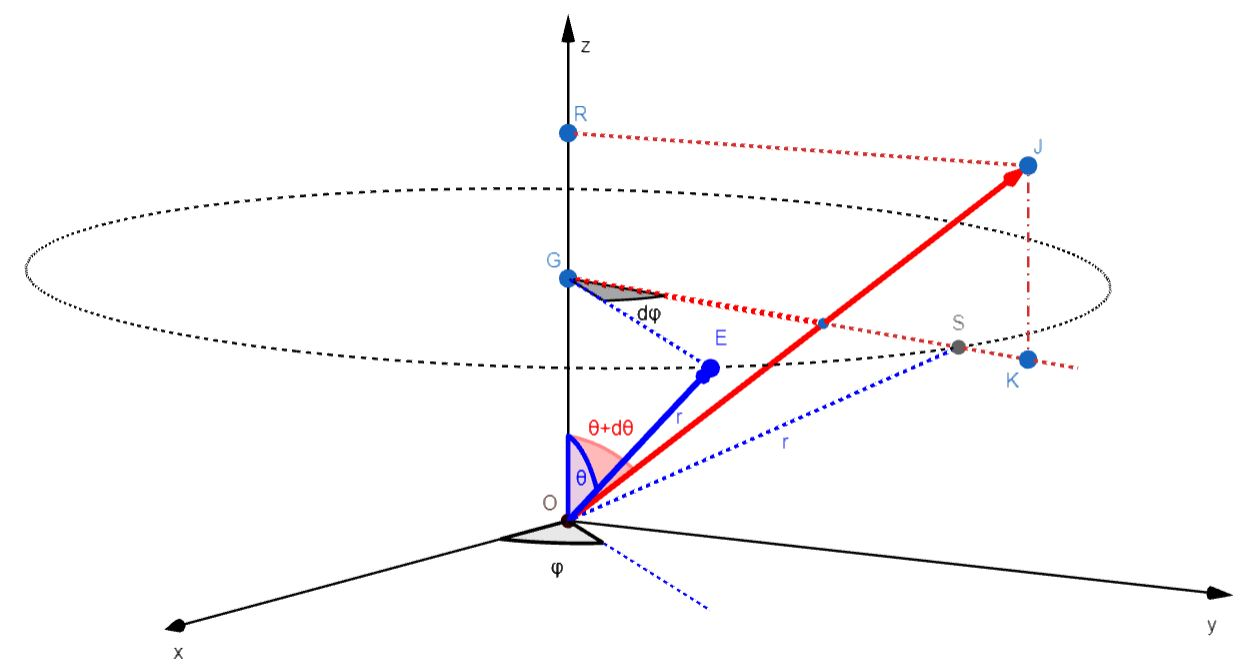
\includegraphics[scale=.5]{sphericalmetric.jpg}
\begin{align}
\ ds^2 &= |EJ|^2
\end{align}
As we use infinitesimal displacements we can assume that $$|ES|\perp|GK|\perp|JK|\perp|ES|$$. Hence,
\begin{align}
\ ds^2 = |ES|^2+|SK|^2+|KJ|^2
\end{align}
We have the following relationships
\begin{align}
\left.
\begin{array}{c}
\ |ES| = r\sin(\phi)d\theta\\\\
\ |GE| = |GS| = r\sin(\phi)\\\\
\ |GK| = |RJ| = (r+dr)\sin(\phi+d\phi) \\
\ =(r+dr)(\cos(\phi)\sin(d\phi)+\sin(\phi)\cos(d\phi) )\\
\ = (r+dr)(\cos(\phi)d\phi+\sin(\phi))\\
\ = r\cos(\phi)d\phi+r\sin(\phi)+\sin(\phi)dr\\\\
\ |OR| =  (r+dr)\cos(\phi+d\phi)\\
\ = (r+dr)(\cos(\phi)\cos(d\phi)-\sin(\phi)\sin(d\phi))\\
\ = (r+dr)(\cos(\phi)-\sin(\phi)d\phi)\\
\ = r\cos(\phi)-r\sin(\phi)d\phi + \cos(\phi)dr\\\\
\ |OG| = r\cos(\phi)\\\\
\ |JK| = |OR|-|OG| = \cos(\phi)dr-r\sin(\phi)d\phi\\\\
\ |SK| = |GK|-|GS| = r\cos(\phi)d\phi+\sin(\phi)dr\\\\
\end{array}
\right\}
\end{align}
\begin{align}
\left.
\begin{array}{c}
\ |ES|^2 = r^2\sin^2(\phi)d\theta^2\\
\ |SK|^2 = r^2\cos^2(\phi)d\phi^2+\sin^2(\phi)dr^2 +2r\cos(\phi)\sin(\phi)drd\phi \\
\ |JK|^2 = \cos^2(\phi)dr^2+r^2\sin^2(\phi)d\phi^2 -2r\cos(\phi)\sin(\phi)drd\phi\\
\end{array}
\right\}
\end{align}
Hence,
\begin{align}
\ ds^2 &= |ES|^2+|SK|^2+|KJ|^2\\
&= \left\{ \begin{array}{c} r^2\sin^2(\phi)d\theta^2 \\ +r^2\cos^2(\phi)d\phi^2+\sin^2(\phi)dr^2 +2r\cos(\phi)\sin(\phi)drd\phi\\+r^2\sin^2(\phi)d\phi^2+\cos^2(\phi)dr^2 -2r\cos(\phi)\sin(\phi)drd\phi\\
\end{array}
\right.\\
\ &\Rightarrow ds^2= dr^2 + r^2d\phi^2 + r^2\sin^2(\phi)d\theta^2
\end{align}
$$\medblackdiamond$$
\pagebreak[4]

\section{p25-clarification 1.34}

\begin{tcolorbox}
Be $E = mc^4$ and given an Euclidean space, prove that ....blalbla
....blalbla
....blalbla
....blalbla

\end{tcolorbox}
bma bla blaa

\begin{eqnarray} 
\sum_{i=100}^{\infty} a_i x^i \\
\sum_{i=100}^{\infty} a_i x^i
\end{eqnarray}
$$\medblackdiamond$$
\pagebreak[4]

\section{p25-exercise}

\begin{tcolorbox}
Be $E = mc^2$ and given an Euclidean space, prove that ....blalbla
....blalbla
....blalbla
....blalbla

\end{tcolorbox}
%\setcounter {equation} {1} %sets the counter to have the specified

bma bla blaa

\begin{equation} 
\sum_{i=0}^{\infty} a_i x^i
\end{equation}
\begin{eqnarray} 
\sum_{i=100}^{\infty} a_i x^i \\
\sum_{i=100}^{\infty} a_i x^i
\end{eqnarray}
$$\medblackdiamond$$
\pagebreak[4]

\section{p25-clarification 1.34}

\begin{tcolorbox}
Be $E = mc^4$ and given an Euclidean space, prove that ....blalbla
....blalbla
....blalbla
....blalbla

\end{tcolorbox}
bma bla blaa

\begin{eqnarray} 
\sum_{i=100}^{\infty} a_i x^i \\
\sum_{i=100}^{\infty} a_i x^i
\end{eqnarray}
$$\medblackdiamond$$
\pagebreak[4]

\section{p25-clarification 1.34}

\begin{tcolorbox}
Be $E = mc^4$ and given an Euclidean space, prove that ....blalbla
....blalbla
....blalbla
....blalbla

\end{tcolorbox}
bma bla blaa

\begin{eqnarray} 
\sum_{i=100}^{\infty} a_i x^i \\
\sum_{i=100}^{\infty} a_i x^i
\end{eqnarray}
$$\medblackdiamond$$
\pagebreak[4]
